\documentclass[a4paper,12pt]{article}
\usepackage[latin1]{inputenc}
\usepackage[spanish]{babel}
\usepackage{graphicx}
\usepackage{amsmath}
\pagestyle{empty}
\setlength{\textheight}{235mm}
\setlength{\textwidth}{168mm}
\setlength{\oddsidemargin}{0pt}

\begin{document}
\mbox{}\vspace*{-45mm}

{\centering
{\small\sc Escuela T�cnica Superior de Ingenieros de Caminos, Canales y
Puertos (Madrid)}\\*[4mm]
{\Large\bf M�todo de los Elementos Finitos}\\*[4mm]
Pr�ctica 2: Estructuras de barras articuladas \\*[4mm]
}

\vspace{3mm}

Utilizando ABAQUS Student realizar un modelo de elementos finitos de la viga Pratt de la figura, obteniendo:

\begin{enumerate}
\item Deformada de la estructura empleando un factor de magnificaci�n que permita una visualizaci�n adecuada de la misma.
\item Obtener la flecha en el centro.
\item Obtener el esfuerzo m�ximo producido por la fuerza y
determinar en qu� barra se produce. 
\end{enumerate}

El m�dulo el�stico del material es $E=230$ GPa y la secci�n transversal
de las barras $A=5.0 \cdot 10^{-3}$ m$^2$.

\begin{center}
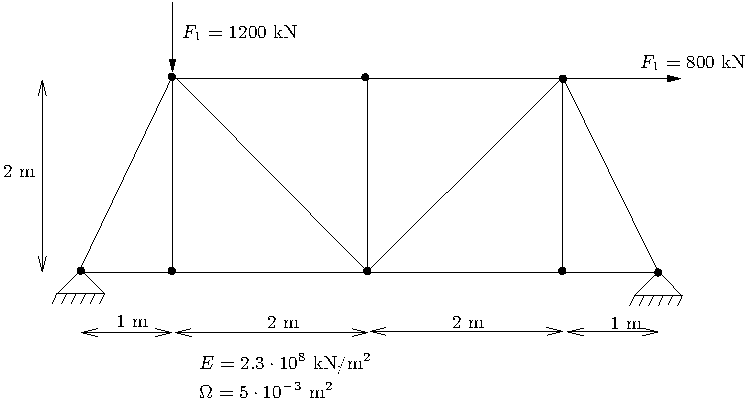
\includegraphics{pract2.pdf}
\end{center}
\end{document}
